\section{Problem Formulation}\label{sec:problem_definition}
Let $S$ denote a set of subjects which are of potential interests to journalists. 
For example, $S$ can refer to all the players or teams in the NBA application.
Let $e_s(t)$ denote an event about subject $s$, where $t$ denotes its timestamp or sequence ID. 
For example, an event can refer to an NBA game a player participated on a certain day. 
Note that we maintain a sequence ID for each subject that is automatically incremented. 
It is possible that the events of different subjects may have the same sequence ID. 
Consecutive events of the same subject can be grouped as a \textit{streak}:

\begin{definition}[Streak~\cite{zhang2014discovering}]
Let $w$ be a streak length, a streak $W_s(t,w)$ refers to $w$ consecutive 
events of subject $s$ ending at sequence $t$, i.e., $W_s(t,w)=\{e_s(t-w+1),..., e_s(t)\}$.
\end{definition}

If a subject $s$ has $|\mathbb{H}_s|$ events, 
then there are $|\mathbb{H}_s|\choose{2}$ possible 
streaks\footnote{This number is derived by constructing a
streak using start and end sequence IDs.
}. 
Given an aggregate function $f$, events in a streak can be aggregated to a numerical value $\overline{v}$ as:
$$W_s(t,w).\overline{v} = f(e_s(t-w+1),..., e_s(t))$$

%In general, if a subject $s$ has $|\mathbb{H}_s|$ events, there are $|\mathbb{H}_s|\choose{2}$ possible event windows. Given an aggregate function $f$, events in an event window can be aggregated to a numerical value $\overline{v}$ as:
%$$W_s(t,w).\overline{v} = f(e_s(t-w+1),..., e_s(t))$$

Common aggregate functions include \emph{sum}, \emph{avg}, \emph{count}, \emph{min} and \emph{max}. 
In this thesis, we only consider a single aggregate function. Multiple aggregate functions can be 
simply  processed independently.
%To support multiple aggregation functions, one may simply invoke our solution multiple times to process them independently.

%We support all the common aggregate functions such as \emph{sum}, \emph{avg}, \emph{count}, \emph{min} and \emph{max}.
%\footnote{Streaks defined in~\cite{zhang2014discovering} only support \emph{min}, \emph{max}, which are special cases of the streaks defined here.}
%For simplicity of presentation,
%We only consider a single aggregate function in our solution. 
%To support multiple aggregation functions, one may simply invoke our solution multiple times to process them independently.

\begin{example}
Figure~\ref{fig:system_flow} (A) illustrates examples of \textit{streak}s of three NBA players. 
Each event records the points scored by a player in a game. 
In the figure, the streak $W_{s_1}(3,2)$ refers to two consecutive events
about player $s_1$ ending at $t=3$, i.e., $W_{s_1}(3,2)=\{e_{s_1}(2), e_{s_1}(3)\}$. 
Given an aggregate function $f=avg(points)$,  we yield $W_{s_1}(3,2).\overline{v}=(46+10)/2=28$.
\end{example}

\begin{figure*}[t]
\centering
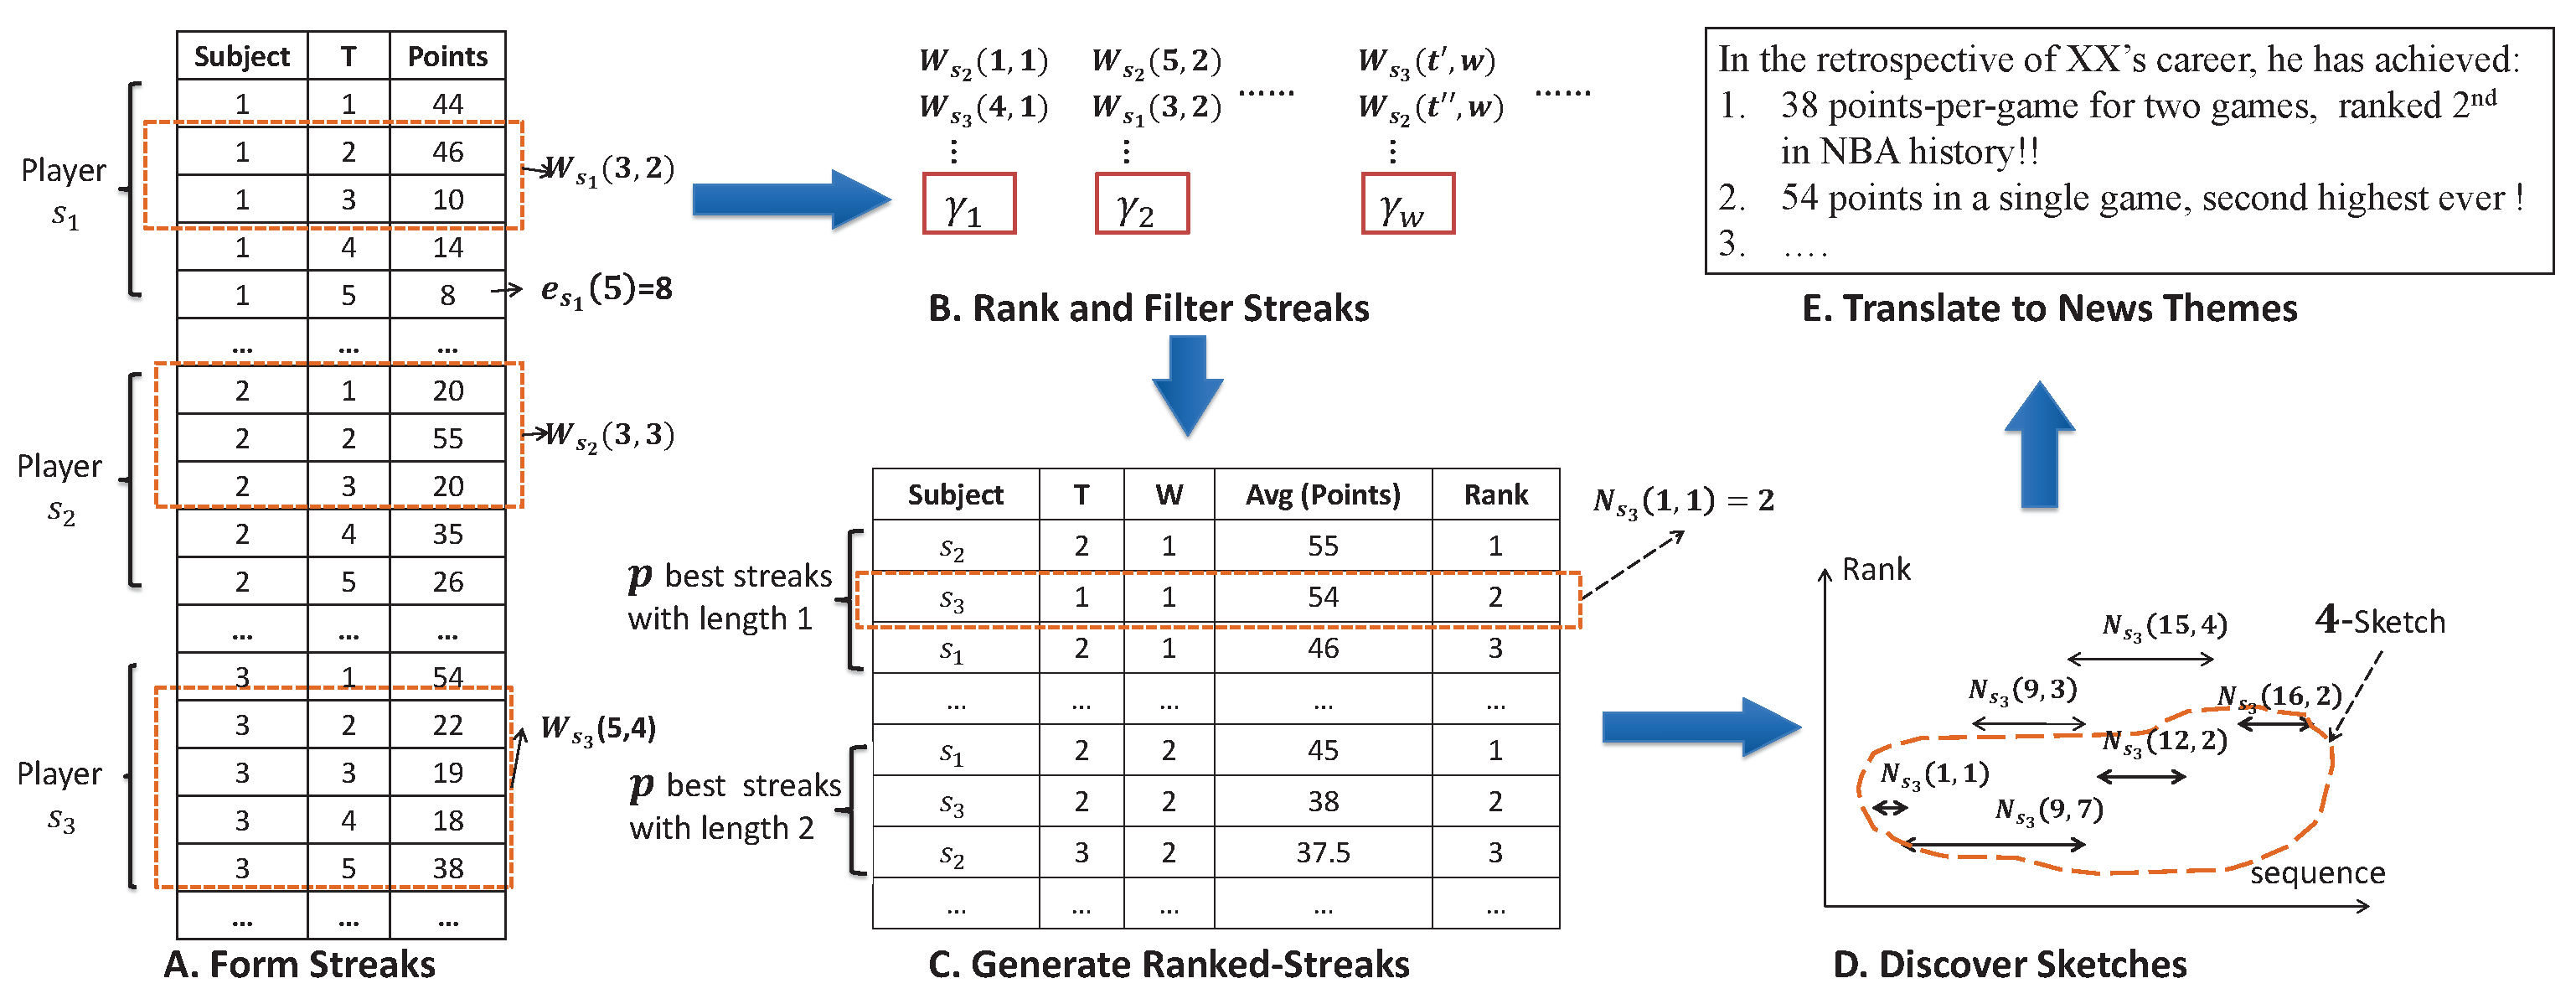
\includegraphics[width=1.0\textwidth]{chapter4/charts/application.eps}
	\caption{An illustration of $k$-Sketch query processing. 
(A): various streaks are formed based on events' sequence IDs. 
(B): streaks with rank greater than $p$ are filtered.
(C): ranked-streaks for each streak length.
(D): $k$-sketches are discovered for each subject from their ranked-streaks.
(E): newsworthy summary of a subject can be generated from its $k$-sketches.
}
\label{fig:system_flow}
\end{figure*}

With the aggregated value $\overline{v}$, we can derive the \emph{rank} of a streak
to measure its strikingness.
%which can be used to measure its strikingness. 
For instance, ``\textit{The total points Kobe has scored is $32,482$}'' can be transformed into a rank-aware representation: ``\textit{Kobe moved into third place on the NBA's all-time scoring list}'', where the rank is $3$. Let $W$ be a length-$w$ streak, and 
 $\gamma_w(W.\overline{v})$ be the rank of $W$ by comparing it with all other
length-$w$ streaks on their aggregate values. 
Let $p$ be a predefined threshold to indicate
whether a streak is striking (i.e., top-$p$). 
These concepts lead to our definition of  \emph{Ranked-Streak}:
%Then, our
%definition of \emph{Ranked-Streak} is formed as follows:

%In general, a streak is striking if its rank is smaller than a predefined threshold (i.e. top-$p$). These lead to our definition of \emph{Ranked-Streak}:

%With the aggregated value $\overline{v}$, we can derive the rank of an event window, which can be used to measure the strikingness of an event window as a news theme.  For instance, ``\textit{The total points Kobe has scored is $32,482$}'' can be transformed into a rank-aware representation: ``\textit{Kobe moved into third place on the NBA's all-time scoring list}'', in which the rank is $3$. Let $W$ be a length-$w$ event window, and 
% $\gamma_w(W.\overline{v})$ be the rank of $W$ by comparing it with all other
%length-$w$ event windows on their aggregate values. Generally speaking, an event window is newsworthy if its rank is smaller than a predefined threshold. This leads to our definition of \emph{Candidate Theme}:
%

\begin{definition} [Ranked-Streak]
A streak $W_s(t,w)$ can be transformed to a ranked-streak, denoted by $N_s(t,w)$, if its rank $\gamma_w(W_s(t,w).\overline{v}) \leq p$, where $p$ is a user-defined threshold.
\end{definition} 

\begin{example}
In step $(B)$ of Figure~\ref{fig:system_flow}, we group the streaks based on their lengths. Each streak is associated with a rank value $\gamma_w$. If the rank is greater than the threshold $p$, the associated streak is pruned. 
Otherwise, it is considered as a ranked-streak. In step $(C)$ of  Figure~\ref{fig:system_flow}, we present the ranked-streaks in the tabular format. Each ranked-streak contains the rank computed from step (B). 
For instance, among all ranked-streaks with length 1, $N_{s_3}(1,1)$ (with value $54$) is ranked 2$^{nd}$ 
because its aggregated value is smaller than that of another streak $N_{s_2}(2,1)$ (with value $55$). %Therefore the rank of $N_{s_3}(1,1).\gamma=2$.
\end{example}

Let $\mathbb{N}_s$ be the set of ranked-streaks of a subject $s$. Since there are at most $p$ ranked-streaks for each possible streak lengths, the size of $\mathbb{N}_s$ can be as large as $p|\mathbb{H}_s|$ which is still overwhelming for 
summarizing the subject's history.
To control the output size while maintaining the quality of the summary, 
we aim to find a subset of $k$ ranked-streaks
%candidate themes 
from $\mathbb{N}_s$ which best summarize the history of $s$. %, which $best$ describes $\mathbb{N}_s$. 
We name such a subset a $k$-\textbf{Sketch}.


To measure the quality of the selected ranked-streaks, we define a scoring 
function $g(\cdot)$. The design of $g$ gives rise to two concerns.
First, $g$ prefers ranked-streaks covering as many of the subject's historical
events as possible. This is because a higher coverage indicates fewer missing historical events in the summary.
Second, $g$ needs to assign a higher score to the ranked-streaks with better ranks. This
is because a better rank indicates higher strikingness which implies that the news themes generated would
be more eye-catching. 
For instance, 
we often care more about who the top scorer in NBA history is rather than who is ranked $50^{th}$.
%
%First, $g$ needs to assign higher scores to the ranked-streaks with better ranks. This
%is because better rank indicates better strikingness which implies that the news themes generated would
%be more eye-catching. 
%For instance, 
%we often care more about who the top scorer in NBA history is rather than who is ranked $50^{th}$.
%Second, $g$ prefers ranked-streaks with fewer overlapped events and penalizes on near-duplicate streaks. 
%This is because near-duplicate streaks generally do not add news values.
%For example, when Kobe Bryant scored 81 points in a single game ($2^{nd}$ highest in NBA history),
%all streaks containing that event are likely to have good and similar ranks. 
%Thus, selecting all of them is not newsworthy.

To address these two concerns, we define $g$ as follows: 
let $\mathbb{X}_s$ be a set of ranked-streaks about subject $s$ (i.e., $\mathbb{X}_s \subseteq \mathbb{N}_s$), 
the score of $\mathbb{X}_s $ is:
\begin{equation}
	\label{eq:scoring_function}
	g (\mathbb{X}_s) = \alpha C(\mathbb{X}_s) + (1-\alpha) R(\mathbb{X}_s), \alpha \in [0,1]
\end{equation}
where $C(\mathbb{X}_s)$ is the ratio between the number of distinct events covered by $\mathbb{X}_s$ 
over the total number of events about subject $s$. In this way, ranked-streaks with a poor coverage
contribute to a low score. $R(\mathbb{X}_s) = \frac{1}{|\mathbb{X}_s|}\sum_{X_s \in \mathbb{X}_s} \frac{p-X_s.\gamma}{p}$ is the strikingness of $\mathbb{X}_s$. Any ranked-streak in 
$\mathbb{X}_s$ changing to a better rank increases $R(\mathbb{X}_s)$. The value ranges of $C(\mathbb{X}_s)$ and $R(\mathbb{X}_s)$ are guaranteed to be in $[0,1]$. $\alpha$ is an adjustable coefficient to balance the weights between $C(\mathbb{X}_s)$ and $R(\mathbb{X}_s)$. If $\alpha$ is high, it means users are more interested in finding ranked-streaks that cover most of the subject's history.  If $\alpha$ is low, it indicates that users prefer more striking ranked-streaks.

With Equation~\ref{eq:scoring_function}, we then define the \emph{$k$-Sketch Query} as follows:

\begin{definition} [$k$-Sketch Query]
Given a parameter $k$, $k$-Sketch Query aims to, for each subject $s$, 
find a subset $SK_s$ from the ranked-streaks of $s$ (i.e., $SK_s \subseteq \mathbb{N}_s$), s.t. $|SK|_s = k$ and $g(SK_s)$ is maximized.
\end{definition}

\begin{example}  
In step $(D)$ of Figure~\ref{fig:system_flow}, we show a collection of ranked-streaks and a $k$-Sketch derived from them. The $y$-axis is the rank and the $x$-axis represents the complete sequence of events of a subject. 
Each ranked-streak is represented by a line segment, covering consecutive events. When $k=4$, four of the ranked-streaks are selected as the $4$-Sketch.%; and they form the $4$ most striking news themes which summarize the subject history.
\end{example}

Before we move on to the algorithmic part, we first list the frequently used notations in Table~\ref{tbl:notations}. For 
ease of presentation, we present our techniques using \emph{avg} as the default aggregate function. Extending our techniques to other aggregate functions is addressed in Section~\ref{sec:discussion}.

\begin{table}[h]
\caption{Notations used in this chapter.}
\centering
\begin{tabular}{|c|l|}  
\hline 
\textbf{Notation} & \textbf{Meaning} \\ 
\hline
$S$ & set of subjects \\
\hline
$\mathbb{H}_s$ & set of events associated with subject $s$\\
\hline
$W_s(t,w)$ & length-$w$ streak of $s$ ending at $t$\\
\hline
$\mathbb{N}_s$ & set of ranked-streaks associated with subject $s$\\
\hline 
$N_s(t, w)$ & the ranked-streak derived from $W_s(t,w)$ \\ 
\hline 
$WI(w)$ & top-$p$ ranked-streaks of length $w$\\
\hline
$\beta(w)$ & lower bound of $WI(w)$\\
\hline
$SK_s$ & sketch for subject $s$ \\
\hline
$J_s$ & visiting-streak bound for subject $s$ \\
\hline
$M_s$ & unseen-streak bound for subject $s$\\
\hline
$P_s$ & online-streak bound for subject $s$\\
\hline
\end{tabular} 
\label{tbl:notations}
\end{table}
